\begin{surferPage}[Con quadràtic]{Con quadràtic}
Es diu que una superfície és \emph{no singular} o \emph{llisa}
si no té, en sentit intuïtiu, punxes, arestes o plecs
(dels quals en diem \emph{singularitats}).
    \vspace{-0.2cm}
    \begin{center}
      \begin{tabular}{@{}c@{}c@{}c@{}c@{}}
        \begin{tabular}{@{}c}
          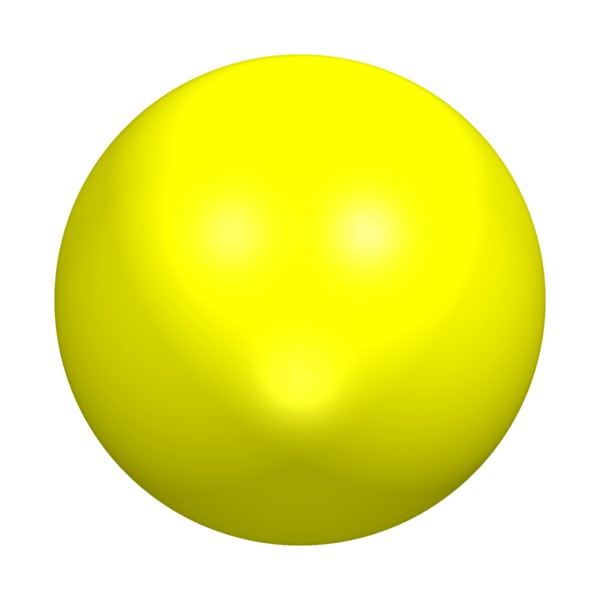
\includegraphics[width=1.1cm]{../../common/images/kugel}
        \end{tabular}
        &
        \begin{tabular}{@{}c}
          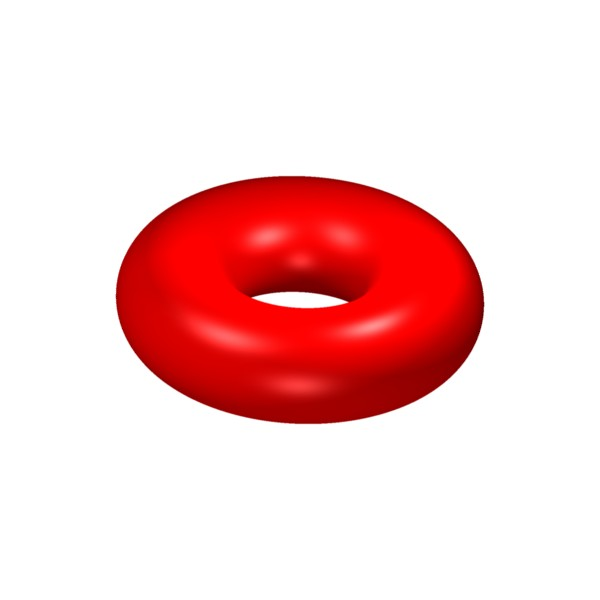
\includegraphics[width=1.1cm]{../../common/images/torus}
        \end{tabular}
        &
        \begin{tabular}{c@{}}
          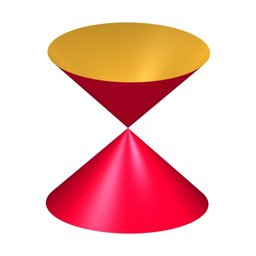
\includegraphics[width=1.1cm]{../../common/images/kegel}
        \end{tabular}
        &
        \begin{tabular}{c@{}}
          \includegraphics[width=1.1cm]{../../common/images/A2pm_ill}
        \end{tabular}
      \end{tabular}
    \end{center}
    \vspace*{-0.4em}
L'esfera o el tor són llises. El con quadràtic té un punt singular
del tipus més simple ($A_1^{+-}$). Si es `deforma' la seva equació
$x^2+y^2-z^2=0$ posant en lloc del 0 un nombre $a$ qualsevol,
la superfície
\[x^2+y^2-z^2=a\]
és llisa si $a\neq0$. Imatges per a $a=-\frac12$, $a=0$, $a=\frac12$:
    %
    \begin{center}
      \begin{tabular}{@{}c@{\quad}c@{\quad}c@{}}
        \begin{tabular}{@{}c@{}}
          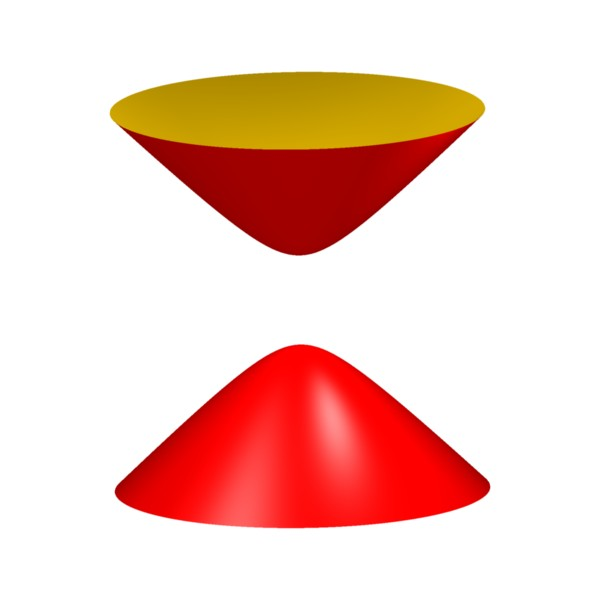
\includegraphics[width=1.2cm]{../../common/images/A1pm_0}
        \end{tabular}
        &
        \begin{tabular}{@{}c@{}}
          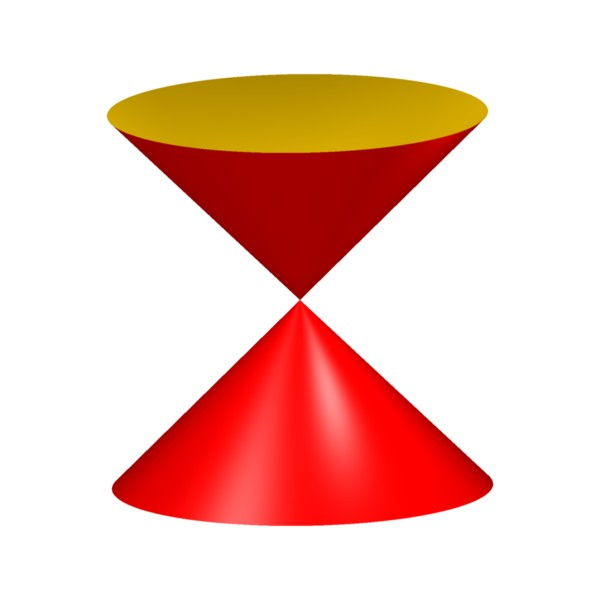
\includegraphics[width=1.2cm]{../../common/images/A1pm_1}
        \end{tabular}
        &
        \begin{tabular}{@{}c@{}}
          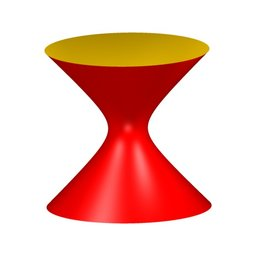
\includegraphics[width=1.2cm]{../../common/images/A1pm_2}
        \end{tabular}
      \end{tabular}
    \end{center}
    \vspace*{-0.4em}
En els exemples que segueixen es veurà que és possible deformar
singularitats més complicades de manera que apareguin un cert
nombre de singularitats com les del con quadràtic (singularitats còniques).
\end{surferPage}
